\chapter{Bulk medium evolution and initial condition}
In this chapter, I shall introduce a hydrodynamic based model for describing the bulk medium evolution in the heavy-ion collision.
After the basic description of the modeling, I will show an application of this simulation framework in reverse engineering the three-dimensional initial entropy deposition, which is one of my published research projects.

\section{A Hydrodynamics-based dynamical modeling}
\subsection{The hydrodynamic equations}
There has been vast experimental evidences that supports the use of an relativistic viscous hydrodynamics in describing the dynamical evolution of the medium created in the heavy-ion collision.
At mid-rapidity, the hydrodynamic-based model can achieve a high precision of agreement with a global comparison to experimental data. 
This data also support the use of a small but nonzero specific shearviscosity {Muronga:2004sf, Chaudhuri:2006jd, Romatschke:2007mq, Dusling:2007gi, Song:2007ux, Luzum:2008cw}, and more recent studies and global Bayesian analysis also suggest the use of a finite bulk viscosity.

\paragraph{Ideal hydrodynamics} Hydrodynamics is a macroscopic description that propagates the energy momentum tensor of the system without an microscopic knowledge of the degrees of freedom.
The first four equations comes from the the energy-momentum conservation,
\begin{eqnarray}
\partial_\mu T^{\mu\nu} = 0
\end{eqnarray}
where $T^{\mu\nu}$ is the energy momentum tensor and $\partial_\mu = \partial/\partial x^\mu$. 
Here we have choose the metric as $g^{\mu\nu} = \diag\{1, -1, -1, -1\}$.
If one assumes ideal hydrodynamics that the system always relax to local thermal equilibrium fast enough compared to other time scale, then $T^{\mu\nu}$ can be expressed as
\begin{eqnarray}
\partial_\mu T^{\mu\nu} = e u^\mu \nu - P (g^{\mu\nu}-u^{\mu\nu})
\end{eqnarray}
where $u^\mu$ is the flow velocity such that in the co-moving frame  $T^{\mu\nu}$ has the diagonal form $T^{\mu\nu} = \diag\{e, -P, -P, -P\}$.
Therefore $e$ and $P$ are the energy density and pressure of the thermalized matter in the rest frame.
There are five unknowns $e, P, u_x, u_y, u_z$ ($u_t$ is determined by $u^2 = 1$), but conservation laws only provide four equations.
A fifth equation is the equation of state (EoS) $P = P(e)$ that encodes thermodynamic properties of the medium (in this case, the nuclear medium at finite temperature) which closes the set of ideal-hydrodynamic equation.
\paragraph{Inputs from first principal calculation} The lattice QCD simulation has determined the QCD equation of state to high precision with physical masses of the light flavor.
It is not a prior known that the lattice QCD EoS computed for an infinite matter in infinite time is the best choice for describing a transient, finite size system, however, using the lattice input does result in reasonable agreement with the data.
Moreover, there has been a study that try to constrain the from of EoS from experimental data and the ``calibrated'' EoS is very close the Lattice prediction.
Most of the currently hydrodynamic studies already uses the state-of-the-art lattice results.
\paragraph{Viscosity correction and QCD transport coefficient}
The medium created in heavy-ion collision undergoes fast longitudinal and transverse expansion, and the thermalization rate may not be fast enough to keep the system in fully thermal equilibrium,
\begin{eqnarray}
T^{\mu\nu} = u^\mu u^\nu e - (g^{\mu\nu}- u^\mu u^\nu) (P+\Pi) + \pi^{\mu\nu}
\end{eqnarray}
Here $T_0$ is the thermal part, and $\pi$ is the shear viscosity correction, and $\Pi$ is the bulk viscosity correction to the pressure.
Relativistic viscosity hydrodynamics that expands the transport description in terms of the Knudsen number is developed to taken into account viscous effects.
At first order, this is well-known Naiver-Stokes equations, where the $\pi$, $\Pi$ are given by the constitutive relations,
\begin{eqnarray}
\pi^{\mu\nu} &=& 2\eta\sigma^{\mu\nu}\\
\Pi &=& -\zeta\theta
\end{eqnarray}
Here the corrections to the energy momentum tensor are proportional to the first gradient of the macroscopic field $\sigma^{\mu\nu} = \partial^{\langle \mu} u^{\nu\rangle}, \theta = \partial\cdot u$.
The proportional constant are known as the (first order) transport coefficient of the QCD matter, which encodes the dynamical information of the system. 
Especially their dimensionless ratio to the entropy density $\eta/s$ and $\zeta/s$ are important indicator of the interaction strength and the scale-violation of the QCD matter and are of great physical importance.
There have been many effort to either computing these quantities from first principles and effective models or extracting these numbers in a model-to-data comparison.
Coming back to the hydrodynamic modeling, it is shown that one has to go to second order in the expansion to the render the correction compatible with special relativity and $\pi$, $\Pi$ becomes dynamical quantities which tends to relax to the Naiver-Stokes limit.
\begin{eqnarray}
\nonumber
\tau_\pi \dot{\pi}^{\langle\mu\nu\rangle}+\pi^{\mu\nu} &=& 2\eta\sigma^{\mu\nu}- \delta_{\pi\pi}\pi^{\mu\nu}\theta + \phi_7 \pi_{\alpha}^{\langle\mu}\pi^{\nu\rangle\alpha}-\tau_{\pi\pi}\pi_{\alpha}^{\langle\mu}\sigma^{\nu\rangle\alpha} + \lambda_{\pi\Pi}\Pi\sigma^{\mu\nu},
\\
\nonumber
\tau_{\Pi}\dot{\Pi} + \Pi &=& -\zeta\theta - \delta_{\Pi\Pi}\Pi\theta + \lambda_{\Pi\pi}\pi^{\mu\nu}\sigma_{\mu\nu}.
\end{eqnarray}
The $\delta, \phi, \lambda$ are known as second order transport coefficients.
This complicated set of equations together with the conservation law and the EoS forms the viscosity hydrodynamic equations.
Nowadays, well tested numerical packages have been developed solving these equations in the context of heavy-ion collisions.

\paragraph{Boost-invariance approximation and beyond}
In general, the hydrodynamic equations have to be solved as a 3+1 dimensional problem.
But a reduction to a 2+1 dimension is possible, if one assume the fast expansion along the beam-axis (longitudinal) direction has an approximated symmetry near mid-rapidity.
This approximate symmetry is first proposed by Bjorken in [] that the system at different rapidity looks similar upto a longitudinal boost, so that one may first obtain the solution to the 2+1 dimension problem at one space-time rapidity ($\eta_s = 0$) and then boost the solution to other $\eta_s$.
A direct consequences of this symmetry is that the observables should not depends on space-time rapidity.
The $\eta_s$-dependence cannot be directly detected, but can be related to the the rapidity / pseudo-rapidity for the reason below.
Suppose that the Lorentz contracted nuclei interact at $z=0$ and produce excitations that free-stream in the longitudinal direction, then for each of these excitation
\begin{equation}
  \frac{z}{t} = \frac{p_z}{E}.
\end{equation}
This approximation the equivalence of $\eta_s$ and $y$ at early stages of the collision:
\begin{equation}
  \eta_s = \frac{1}{2}\log\frac{t+z}{t-z} \sim y = \frac{1}{2}\log\frac{E+p_z}{E-p_z}.
\end{equation}
If one further assumes these initial excitations are mass-less partons, then the rapidity can be approximated by pseudorapidity as $E\approx |p|$.
The event-averaged rapidity-distribution of charged particles $dN_{\textrm{ch}}/dy$ in both proton-proton and symmetric nuclei-nuclei collisions at the LHC energy falls at large rapidity but has a slowly varying profile at mid-rapidity within $|y|<2$, which is a motivation to apply the boost-invariant at mid-rapidity as a first approximation.

However, since $dN_{\textrm{ch}}/dy$ are event-averaged quantities, its being flat within $|y|<2$ does not rule out that event-by-event particle production fluctuation can break the approximation, and these fluctuations, local in transverse plane, can be different at different transverse location.
Moreover, asymmetric nuclear collision such as $p+Pb, p+Au, d+Au, He+Au$, etc clearly breaks the boost-invariance even on an event averaged level. 
Therefore, the study of longitudinal fluctuation related observables or the search for hydrodynamic  behavior in small collision system clearly requires one to go beyond the boost-invariance approximation.

\subsection{Particularization and microscopic transport}
The longitudinal expansion and the transverse expansion driven by the pressure difference cools down the system temperature and density rapidly and eventually the relaxation rate is too low for the the hydrodynamic approach to apply.
When this happens, one can switch to the microscopic transport description of the system.
This switching is usually done near or below the pseudo-critical temperature $T_{sw} \lesssim T_c$ so that the energy momentum tensor can be particularized as an ensemble of hadrons .
This choice $T_{sw} \lesssim T_c$ avoids the problem of modeling quark / gluon dynamics and hadronization in the strong coupled regime near $T_c$, and whether a hydrodynamics with lattice EoS and a hadronic transport model with cross-sections as inputs are both valid in this regime is another question.
The hydrodynamic $T^{\mu\nu}$ is usually particlized at a constant energy density / temperature hypersurface using the Cooper-Frye formula,
\begin{eqnarray}
dN_i^a(p) = \frac{g^a f^a(p) dp^3}{(2\pi)^3}  \frac{p^{\mu}}{E} \Delta \sigma_{i,\mu} 
\end{eqnarray}
Where the particle yield of specie ``$a$'' with momentum $p$ from the $i^{\textrm{th}}$ surface element $\sigma_{i,\mu}$ equals its phase space density times the surface area (with units of a 3D volume) parallel to the  four velocity $p^\mu/E$.
This distribution function should include both a thermal part and a viscous correction, $f = f_0 + \delta f$.
There are more than one way to construct the viscous correction $\delta f$  from $e, P, n, \Pi$ and $\pi^{\mu\nu}$ based on different assumptions of the form of corrections.
In this work, we shall use a non-additive $\delta f$ correction that has been developed and implemented by [] and [], and please refer to the references for the original formulation and numerical implementations details.

The particlized hadronic system is then solved by the Ultra-relativistic Quantum Molecular Dynamics (UrQMD) model until the system is dilute enough and interactions ceases (kinetic freezeout). 
The UrQMD in the context of hadronic cascade (afterburner) includes processes like resonance decays, elastic and inelastic scatterings, and string formations and fragmentations.

\subsection{Pre-equilibrium stage}
At very early times of the collision, the system is off equilibrium. 
However, viscous hydrodynamic assumes a closeness to the local thermal equilibrium  (there are also recent efforts in studying the effectiveness of hydrodynamics outside of its traditional range of application []).
A successful prediction using an early onset of hydrodynamic evolution at $\tau_0\lesssim 1$fm/$c$ suggests a fast hydrodynamization, whose exact mechanism is still a debatable question. 
There are different modelings of this pre-equilibrium stage, including solving the classical Yang-Mills equation [], partonic transport models [], a collision-less Boltzmann equation [], and the linear response method of the effective kinetic approach [].

Such a pre-equilibrium stage was not included in my study of the 3D initial condition, where the simulation starts at $\tau_0 = 0.6$ fm/$c$ assuming local thermal equilibrium.
For my later study of the heavy flavor dynamics, a 2+1D collision-less Boltzmann equation implemented by [] was later used in obtaining the medium evolution history.
In such a model, the initial energy density ($\tau = 0^+$) at mid-rapidity  is thought to be carried by mass-less partons that propagates at the speed of light in the transverse direction. 
The initial distribution function is assumed to have a factorized form $f(x_\perp, p_\perp, \tau=0) = n(x, \tau=0) \times dN/dp_\perp^2$.
The momentum distribution $dN/dp_\perp^2$ do not evolve as the collisions are neglected, while the spatial density evolves as
\begin{eqnarray}
n(\vec{x}, \tau) = \int n(\vec{x}', \tau=0) \delta^{(2)}(\vec{x} - \vec{x}'- \tau) d\vec{x}'^2
\end{eqnarray}
Then, the model assumes a sudden hydrodynamization at time $\tau_{\textrm{hydro}}$, where the free-streamed,
\begin{eqnarray}
T^{\mu\nu}(x_\perp, \tau_{\textrm{hydro}}) = \int f(x_\perp, p_\perp, \tau=0) \frac{p^\mu p^\nu}{E} dp^3
\end{eqnarray}
is used for initializing the hydrodynamic equations by the Landau matching procedure [].

\section{Initial condition model}
Unlike the dynamical models that are governed by a few equations / laws with a few parameters, the initial condition model parameterizes many more unknowns.
For different initial condition models, these unknowns can be initial color density of the nuclear wave function, the effective size of a nucleon, the form factor of nucleon-nucleon inelastic cross-section, and the amount of fluctuations in particle production / energy deposition, etc.
There are two classes of initial condition models:
\begin{itemize}
\item Models that takes into the particle production dynamics. Such as minijet production, strings productions and flux-tubes, hadronic transport,and color-glass condensate (CGC) effective field theory based models {Wang:1991hta, Zhang:1999bd, Werner:2010aa, Petersen:2008dd, Schenke:2016ksl, Dumitru:2011wq, Hirano:2012kj}.
\item Parametric models that provides macroscopic initial conditions without a dynamical component. Such as Monte-Carlo Glauber models and its extensions [Bozek:2015bna], and the \trento model to be explained [Scott].
\end{itemize}
I shall focus on the development of a parametric model \trento to help the understanding of the initial three-dimensional entropy deposition.


\subsection{The original (boost-invariant) \trento\ model}
The original \trento\ model is proposed as a flexible ansatz to investigate a family of entropy / energy deposition behaviors at mid-rapidity.

First, the impact parameter $\vec{b}_{AB}$ between the two colliding nuclei $A$ and $B$ is sampled at random.
Then, the 3D nucleons positions inside each nuclei are sampled according to the Woods-Saxon distribution (for heavy nuclei, for light nuclei such as Deuteron, Helium, Oxygen where the nucleon distribution is not well approximated by a Woods-Saxon form, the sampling are different),
\begin{eqnarray}
\frac{df_N}{r^2 dr d\phi d\cos\theta} = \frac{1}{\exp\{\frac{r-R(1+\beta_2 Y_{20}(\theta)+\beta_4 Y_{40}(\theta))}{a}\}+1}
\end{eqnarray}
including the quadrupole and hexadecapole deformation of certain nuclei.
The randomized nucleon position is critical to explain the odd order of flow harmonics observed in experiments [].

Then, the collision between the two nuclei is analyzed at the nucleon level. 
Every nucleon pair $\{i, j\}$ with $i$ from nuclei $A$ and $j$ from nuclei $B$ has a certainty probability to undergo an inelastic collision, given the impact parameter $\vec{b} = \vec{b}_{AB} + \vec{x}_{i, \perp} -  \vec{x}_{j, \perp}$,
\begin{eqnarray}
P(b; \sigma) = 1 - \exp\left[-\sigma T_{pp}(b)\right],
\label{dsigma_db}
\end{eqnarray}
where $T_{pp}(b)$ is the overlapping function between the density of the nucleon,
\begin{eqnarray}
T_{pp}(b) = \int d\vec{x}_\perp^2 T_p(\vec{x}_\perp-\vec{b}/2) T_p(\vec{x}_\perp+\vec{b}/2)
\end{eqnarray}
And each nucleon is assumed to have a Gaussian density profile, 
\begin{eqnarray}
T_p(\vec{x}_\perp^2) = \frac{1}{2\pi w^2} \exp\left(-\frac{\vec{x}^2}{2w^2}\right)
\end{eqnarray}
with the width of the nucleon $w$ a free parameter.
The $\sigma$ is an effective constituent cross-section that is determined by reproducing the experimental measured proton-proton inelastic cross-section at a given beam energy,
\begin{eqnarray}
\sigma_{pp}^\text{inel}(\sqrt{s}) = \int d\vec{b}^2 P(b; \sigma(\sqrt{s}))
\end{eqnarray}
Applying the probabilistic collision criteria of equation \ref{dsigma_db} to each pair of nucleons, the nucleons that suffer at least one inelastic collisions are called participant and the total number of binary inelastic collisions are denoted as $N_{\textrm{bin}}$.
The minimum-biased event sample in the \trento model are defined all events that has at least one binary collision, 

The above procedure is similar to the that of an Monte-Carlo Glauber model in determine the nuclear inelastic cross-section.
The key step of \trento is an ansatz that maps from the participants in a particular event to the energy / entropy density deposited at the mid-rapidity.
We fist define the participant densities,
\begin{equation}
T_{A, B}(\x) = \sum_{i\in \textrm{Parts}_{A, B}} w_i\, T_p(\x - \x_i).
\end{equation}
The summation goes over the participants in nuclei $A$ and $B$, and each participant contribute a fluctuating contribution proportional to its transverse density $T_p$.
The fluctuating weight $w_i$ follows a $\Gamma$-distribution with unit mean and variance $1/k$ where $k$ is a parameter.
This fluctuating contribution is put in to mimic the multiplicity fluctuation in the proton proton collisions.
The entropy / energy density deposit at mid-rapidity is assumed to be a function of $T_A$ and $T_B$ only at each transverse location,
\begin{eqnarray}
\frac{dS(\vec{x})}{d\eta dx_\perp^2} \textrm{ or } \frac{dE(\vec{x})}{d\eta dx_\perp^2} = f(T_A(\vec{x}), T_B(\vec{x})).
\end{eqnarray}
This simplification is possible because at $\tau=0^+$, causality requires that the entropy production at one location cannot be correlated with the information at a different transverse location. 
Also, the partons that contribute to the bulk low-$p_T$ particle production at high $\sqrt{s}$ are predominately low energy gluons whose longitudinal wavelength is longer than the contracted proton radius in the $z$-direction; therefore, the entropy production should not be sensitive to the details of how the participants aligned but only its $z$-integrated density.
\trento\ parametrizes this mapping from $T_A$ and $T_B$ to the energy / entropy deposition using a ``generally mean'' ansatz,
\begin{eqnarray}
f(T_A, T_B; p) = \left(\frac{T_A^p + T_B^p}{2}\right)^{1/p}.
\end{eqnarray}
$p$ is a tunable parameter and with a few special values, it reduces to the well known average procedures as in table \ref{tab:trento-p}
\begin{table}
\centering
\caption{\trento\ $p$-parameter}\label{tab:trento-p}
\begin{tabular}{ccc}
\hline
$p\in \mathbb{R}$ & $f(x, y)$ & Entropy / energy production\\
\hline
$-\infty$ & $\min\{x, y\}$ &  dominated by the thinner target\\
$-1$ & $2xy/(x+y)$ &   the harmonic mean scaling\\
$0$ & $\sqrt{xy}$ &  the geometric mean scaling\\
$1$ & $(x+y)/2$ &  the arithmetic mean (participant) scaling\\
$+\infty$ & $\max\{x, y\}$ &  dominated by the thicker target \\
\hline
\end{tabular}
\end{table}
This way the model is able to parametrize a class of entropy / energy production scheme and includes certain type of initial condition uncertainty.
Through a global model-to-data comparison, this $p$ parameter has been calibrated to be very close to 0, suggesting the data favors a mid-rapidity entropy / energy deposition that scales as $(T_A T_B)^{0.5}$.
A similar scaling is also found in the EKRT initial condition model based on pQCD plus saturation physics.

\subsection{Parametrize the longitudinal dependence in \trento}
The \trento\ model has been doing successful phenomenology for obserables at mid-rapidity [].
My later work focus on extending the parametrization to a rapidity-dependent initial condition, and seek for a reverse-engineered 3D entropy production from the rapidity-dependent observables.

One constrain in extending the model is that it should reduces to the boost-invariant version of the model at mid-rapidity; therefore, I take the following decomposition of $s(\x, \eta_s)$ at the hydrodynamic starting time $\tau_0 = 0.6$ fm/c,
\begin{equation}
  s(\x, \eta_s)\vert_{\tau=\tau_0} \propto f(T_A(\x), T_B(\x)) \times g(T_A(\x), T_B(\x), \eta_s),
  \label{factorized}
\end{equation}
$f$ is the entropy production at midrapidity as explain above.
Now $g$ parametrize the rapidity-dependence and is always normalized such that $g(T_A(\x), T_B(\x)), 0)=1$.
Qualitatively, the breaking of boost-invariance can come from the initial asymmetry of the incoming nuclear matter $T_A \neq T_B$ and various sources of fluctuation in particle production.
We listed the sources of these contributions and indicated what contribution has been included and what is not,
\begin{itemize}
\item In asymmetric collisions like $p$-$A$ and non-central $A$-$A$, the local thickness functions are imbalanced $T_A \neq T_B$.
\item Even in central $A$-$A$ collision, nuclear / nucleon configuration fluctuations also contribute to the asymmetry. These are included as the randomized nucleon position fluctuation and the $\gamma$-fluctuation of the nucleon thickness function.
\item Initial stage dynamical evolution which can introduce dynamical fluctuations and non-vanishing flow in the $z$-direction is not included.
\end{itemize}
Therefore, the asymmetry in the extended \trento\ model only comes from the imbalanced and fluctuating participant density function.
We parametrize this function in terms of rapidity and then transformed to the space-time rapidity.
\begin{eqnarray}
g(\x, \eta) &=& g(y; T_A(\x), T_B(\x)) \frac{J \cosh \eta_s}{\sqrt{1 + J^2 \sinh^2 \eta_s}},
\label{jacobian}
\end{eqnarray}
where the species-dependent factor $J$ is replaced with an effective value $J \approx \langle p_T \rangle / \langle m_T \rangle$.
Instead of determining a single number at mid-rapidity, we need to map $T_A$ and $T_B$ to a function $g(y; T_A(\x), T_B(\x))$ that has infinite degrees of freedom.
To do these, we choose to parametrize how the $y$-cumulents of $g$ changes with $T_A$ and $T_B$, and reconstruct the function using its first few cumulants (mean $\mu$, standard deviation $\sigma$, and skewness $\gamma$)
\begin{eqnarray}
g(\x, y) &=& \mathcal{F}^{-1}\{\tilde{g}(\x, k)\}, \\
\log \tilde{g} &=&  i \mu k - \frac{1}{2}\sigma^2 k^2 - \frac{1}{6} i \gamma \sigma^3 k^3  e^{-\frac{1}{2}\sigma^2 k^2} + \cdots \label{cgf}
\end{eqnarray}
where for the skewness term, we have included an exponential that systematically includes higher order cumulants to regulate the behavior of the function at large $y$.
Numerically, we have found that within the range of $|y| < 3.3\sigma$, the reconstructed function has a good behavior and remains positive definite.

The remaining task is to parametrize the way these cumulants depends on the participant density,
\begin{itemize}
\item For the mean parameter, we assume it is proportional to the center-of-mass rapidity of the local incoming nuclear matter $\mu = \mu_0\eta_\text{cm}$,
\begin{equation}
  \eta_\text{cm}=\frac{1}{2} \log \left[\frac{T_A e^{y_b}+T_Be^{-y_b}}{T_A e^{-y_b}+T_B e^{y_b}}\right]
\end{equation}
where $y_b$ is the beam rapidity.

\item For the standard deviation, currently we leave it as a global parameter independent on the transverse location $\sigma = \sigma_0$, but only a function of the center-of-mass energy.
\item Finally, for the skewness, there is no clear reason to choose a particular form, so we tested two parametrizations. And in the end, we will check whether the 3D initial condition extracted from data is sensitive to the different choice of parametrizations.
These two choices are termed ``relative skewness'' and ``absolute skewness''.
\begin{itemize}
\item The ``relative skewness'' parametrization assume a skewness proportional to the relative difference of $T_A$ and $T_B$,
\begin{equation}
  \mathcal{A}(T_A, T_B) = \gamma_r\frac{T_A - T_B}{T_A + T_B},
\end{equation}
\item The ``absolute skewness'' parametrization assume a skewness proportional to the direct difference of $T_A$ and $T_B$,
\begin{equation}
  \mathcal{A}(T_A, T_B) = \gamma_a \frac{T_A - T_B}{T_0},
\end{equation}
where a unit for thickness function $T_0=1$~fm$^{-2}$ restores dimensionless of the $\gamma$ parameter.
\end{itemize}
\end{itemize}
We have summarized the two parametrizations in table \ref{tab:parametrization}, and $\mu_0$, $\sigma_0$, $\gamma_r$ or $\gamma_a$, along with the effective Jacobian $J$ are the four additional parameters one introduced for the three-dimensional extended \trento model.
\begin{table}
\centering
\caption{Table}\label{tab:parametrization}
\begin{tabular}{lccc}
\paddedhline
Model & mean $\mu$ & std.\ $\sigma$ & skewness $\gamma$ \\
\paddedhline \noalign{\smallskip}
Relative  & $\frac{1}{2} \mu_0 \ln\left(\frac{T_A e^{y_b}+T_B e^{-y_b}}{T_A e^{-y_b} + T_B e^{y_b}}\right)$ & $\sigma_0$ & $\gamma_r \dfrac{T_A - T_B}{T_A + T_B}$ \smallskip\\
Absolute & $\frac{1}{2} \mu_0 \ln\left(\frac{T_A e^{y_b}+T_B e^{-y_b}}{T_A e^{-y_b} + T_B e^{y_b}}\right)$  & $\sigma_0$ & $\gamma_a (T_A - T_B)/T_0$\smallskip\\
\paddedhline 
\end{tabular}
\end{table}

In figure \ref{fig:3d-example}, we show two sample events from a $Pb$-$Pb$ collision (top plots) and a $p$-$Pb$ collision (bottom plots) generated by \trento\ .
The 3D initial entropy densities are sliced at mid-rapidity $\eta_s=0$ (left plots) and at the $x=0$ plane (right plots).
The mid-rapidity results are identical to the one predicted in the original \trento\ model.
The model is capable of generating fluctuating longitudinal structures that are local in the transverse plane, and breaks the boost-invariance both locally and globally.
For the $p$-$Pb$ event, one can clearly sees that one hot spot extends into the proton going side $\eta_s >0$, while the participant clusters from the lead nuclei pushes the entropy production into the lead going side $\eta_s <0$.

\begin{figure}
\centering
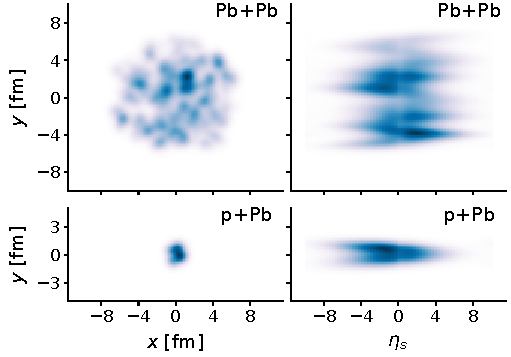
\includegraphics{trento3d_example}
\caption{Initial entropy density in sample Pb+Pb (upper) and p+Pb (lower) events for cross sections of the $\eta=0$ and $x=0$ planes (left and right columns). Event is constructed using the relative skewness model in Table~\ref{tab:parametrization} with $\mu_0=1$, $\sigma_0=3$ and $\gamma_0=6$ along with midrapidity parameters from {Bernhard:2016tnd}.}
\label{fig:3d-example}
\end{figure}

\section{Reverse engineering the 3D initial condition}
In the final section of this chapter, I shall demonstrate applying both the hydrodynamic-based bulk simulation and the flexible \trento-3D initial condition to reverse engineer the 3D entropy deposition at the onset of hydrodynamics at the LHC energies.
Experimentally, one can only measure rapidity-dependent observables on an event averaged level, which already integrates the contribution of particle production over the transverse plane; while our parametrization in the \trento\ model only involves local functions of the participant density function.
Therefore, it is indeed a nontrivial task to infer the functional form of local entropy production $s(\x, \eta_s)$ from these ``global'' measurements.
The suitable statistical technique for parameter inference is the Bayesian 
analysis, which will be introduced in a great detail in chapter \ref{}.

\subsection{Sensitive observables to the initial entropy deposition}
\paragraph{The single particle spectra}
The most direct observable is the charged particle pseudo-rapidity density $\dnchdy$ measured for different collision systems and centralities.
The ALICE collaboration and the ATLAS collaboration has measured this quantity for both $Pb$-$Pb$ system ($-3.5<\eta<5.0$) and $p$-$Pb$ system ($|\eta| < 2.7$) {Abbas:2013bpa,ALICE:2015kda,Aad:2015zza}.
$\dnchdy$ can very well constrain the global rapidity profile and the centrality dependence of the mode, while the limitation being that it is less sensitive to the amount of longitudinal fluctuation.

\paragraph{Two particle pseudo-rapidity correlation}
A good probe of event-by-event longitudinal fluctuations is the two-particle pseudorapidity correlation observable $C(\eta_1, \eta_2)$,
\begin{eqnarray}
C(\eta_1, \eta_2) = \frac{ \left\langle N(\eta_1)N(\eta_2) \right\rangle}{\left\langle N(\eta_1)\right\rangle\left\langle N(\eta_2) \right\rangle}
\end{eqnarray}
The long range part of $C(\eta_1, \eta_2)$ can be shown to sensitive to initial state.
This is because correlation between particles separated by a large gap at proper time $\tau$ in rapidity can only come from proper time before $\tau e^{-|\eta_1-\eta_2|/2}$ even if the information travels at the speed of light.
For example, if one assumes the two particles separated by 4 units of rapidity are emitted at a constant $\tau = 8$ fm/$c$ hydrodynamic freeze-out hyper-surface and neglects the long range correlation that is built by the hadronic cascade, then any correlation must have come from before the proper time $ 8 e^{-2}\approx 1$ fm/c.

To see how $C(\eta_1, \eta_2)$ is related to the longitudinal fluctuation of the entropy deposition / particle production, we follow the analysis in  {Bzdak:2012tp, Jia:2015jga, ATLAS:2015kla} to decompose $\dnchdy$ for each event in a finite pseudo-rapidity window $[-Y, Y]$ using the normalized Legendre polynomials basis,
\begin{eqnarray}
T_n(x) &=& \sqrt{n + \frac{1}{2}} P_n(x)
\end{eqnarray}
And the event-wise charged particle distribution is then,
\begin{eqnarray}
\frac{dN}{d\eta} &=& \biggl\langle\frac{dN}{d\eta}\biggr\rangle \biggl[1 + \sum_{n=0}^\infty a_n T_n\left(\frac{\eta}{Y}\right) \biggr]
\end{eqnarray}
Where $\biggl\langle\frac{dN}{d\eta}\biggr\rangle$ is the reference multiplicity at mid-rapidity for an ensemble of events.
$a_0$ is the total multiplicity fluctuation and $a_1$ controls how the multiplicity distribution is tilted in rapidity in each event and so on.
Two-particle correlation $C(\eta_1, \eta_2)$ measures the variance of these $a_n$ coefficients.
Define the normalized event-wise distribution $R(\eta) = dN/d\eta /\langle dN/d\eta\rangle$, then the two particle correlations can be expressed as the event averaged products of $R$.
\begin{eqnarray}
C(\eta_1, \eta_2) &=& \left\langle R(\eta_1) R(\eta_2)\right\rangle \\
&=& 1 + \sum_{m, n}\langle a_m a_n\rangle  T_{mn}(\eta_1, \eta_2)
\end{eqnarray}
with $T_{mn}$ defined as,
\begin{eqnarray}
T_{mn}(\eta_1, \eta_2) &=& \frac{T_n(\eta_1)T_m(\eta_2) + T_m(\eta_1)T_n(\eta_2)}{2}.
\end{eqnarray}
Therefore, $
\langle a_m a_n\rangle$ can be extracted from two particle correlation.
Combinations like $\langle a_0 a_n\rangle$ reflects how the event-wise rapidity fluctuation correlates with multiplicity fluctuation, which can is canceled to first order by another normalization and define,
\begin{eqnarray}
 C_N(\eta_1, \eta_2) &= \frac{C(\eta_1, \eta_2)}{C_1(\eta_1)C_2(\eta_2)}\\
\end{eqnarray}
with the marginalized function,
\begin{eqnarray}
C_{1,2}(\eta_{1,2}) &= \int_{-Y}^{Y}C(\eta_1, \eta_2)\frac{d\eta_{2,1}}{2Y}.
\end{eqnarray}
And $C_N$ is directly related to the rapidity fluctuation of particle production,
\begin{eqnarray}
C_N(\eta_1, \eta_2) \sim 1 + \frac{3}{2}\langle a_1 ^2 \rangle \frac{\eta_1\eta_2}{Y^2} + \cdots.
\end{eqnarray}
and we shall focus on the $\langle a_1 ^2 \rangle$, which quantifies the amount of linearly-tilting fluctuation.

In additional to the initial condition fluctuation, short range correlation also contributes to the $a_1$ fluctuation {Denicol:2015bnf, Monnai:2015sca}.
The UrQMD hadronic afterburner is able to model certain type short range correlation coming from resonance decay and collisions, but jet-like correlations is hard to accounted for.

\subsection{Calibration of the 3D initial condition parameters}
The degrees of freedom of the initial condition model are,
\begin{itemize}[itemsep=0pt]
  \item[1--2.] Two normalization factors for Pb+Pb and p+Pb collisions at $\sqrts=2.76$~TeV and 5.02~TeV beam energies. they are not fully independent as the $N_{\textrm{p+Pb}} > N_{\textrm{Pb+Pb}}$ is always imposed in the parameter sweep because one expected more particle production is associated to the same thickness function at higher center-of-mass energy.
  \item[3.] The generalized mean parameter $p$ which modulates entropy deposition at midrapidity,
  \item[4.] A gamma shape parameter $k$, which controls the variance of proton-proton multiplicity fluctuations,
  \item[5.] A Gaussian nucleon width $w$, which determines initial state granularity;
  \item[6--8.] Three coefficients which modulate the local rapidity distribution's shift $\mu_0$, width $\sigma_0$, and skewness $\gamma_0$,
  \item[9.] A Jacobian factor $J$ for the conversion from rapidity to pseudorapidity.
\end{itemize}
And the range of the parameters is shown in \ref{tab:trento:parameters}.
One may notice that we did not use different width parameters for the rapidity distribution $\sigma_0$ for $Pb$+$Pb$ and $p$+$Pb$ collisions, though there are different beam energy.
We made this simplification because the the beam rapidity changes less than $8\%$ from $2.76$ TeV to $5.02$ TeV.

\begin{table}
\centering
\caption{Three-dimensional initial condition parameters}
\label{tab:trento:parameters}.
\begin{tabular}{lll}
      Parameter & Description	& Range \\
      \paddedhline
      $N_{\textrm{p+Pb}}$    & Overall p+Pb normalization      & 140.0--190.0 \\
      $N_{\textrm{Pb+Pb}}$   & Overall Pb+Pb normalization     & 150.0--200.0  \\
      $p$	                   & Generalized mean parameter      & -0.3--0.3 (with a prior)  \\
      $k$	                   & Multiplicity fluct.\ shape      & 1.0--5.0  \\
      $w$	                   & Gaussian nucleon width     & 0.4--0.6  \\
      $\mu_0$                & Rapidity shift mean coeff.\     & 0.0--1.0  \\
      $\sigma_0$             & Rapidity width std.\ coeff.\    & 2.0--4.0  \\
      \multirow{2}{*}{$\gamma_0$}             & \multirow{2}{*}{Rapidity skewness coeff.\ }      & 0.0--10.0 (rel) \\
                  &        & 0.0--3.6 (abs)  \\
      $J$	                   & Pseudorapidity Jacobian param.  & 0.6--0.9
\end{tabular}  
\end{table}

The dynamical model consists of both a 3+1D relativistic hydrodynamics and the hadronic afterburner.
The equation-of-state (EoS) is obtained by interpolating a state-of-the-art lattice-QCD EoS {Bazavov:2014pvz} at high temperature (zero baryon density) to a hadron resonance gas EoS at low temperature.
The energy density at which hydrodynamic energy momentum tensor is particulized into hadrons is $\epsilon_{sw} = 0.322$~GeV/fm$^3$ corresponding to a switching temperature close to the pseudo-critical temperature $T_{sw} \sim T_c = 0.154$~GeV).
As a remark, the relativistic hydrodynamics code \mbox{vHLLE} {Karpenko:2013wva} includes the viscous correction, bu we used its ideal mode in the parameter extraction.
This is because the parameter optimization process requires generating running the model on order hundreds different parameter sets.
For each parameter set, thoudands of minimum-biased events needed to be gerenated to achieve a good control of the statistical fluctuation, especially for the correlation observable. 
The full 3+1D viscous hydrodynamics is extremely time consuming, therefore we choose to ran the hydrodynamic model in its ideal mode and on a rather coarse grid.
While the justification is that the rapidity distribution of the multiplicity and normalized two-particle correlations is less sensitive to the viscous effect.
In the end, as a validation to this procedure, we will be using a set of high-likelihood parameter set and run the dynamical model with the viscous correction to see if other observables such as the harmonic flow, and event-plane decorrelations can be reasonably described.


Eventually, four thousands $Pb$+$Pb$ and ten thousands $p$+$Pb$ events 100 are generated at $100$ set of parameter sets.
The computed $\dnchdy$ and $a_1$ fluctuation are computed at differnet centrality, and then the Bayesian analysis makes inference on the probability distribution on the parameters by comparing to measurements.


To investigate the performance of the calibrated models, we show in Fig.~\ref{fig:post_obs} the resulting observables calculated from each model's calibrated emulators.
The bands are centered around the mean prediction, and their spread denotes $\pm 2$ standard deviations.
Both calibrated models are able to simultaneously describe $\dnchdy$ for the two collision systems as functions of rapidity and centrality, illustrating the flexibility of the generating function approach.

The results for rms $a_1$ are compared to preliminary data from ATLAS {ATLAS:2015kla} in Fig.~\ref{fig:post_obs}.
Both models capture the increasing trend of rms $a_1$ as function of centrality.
Hybrid model calculations agree with experimental measurements within $20\%$ for $0$--$50\%$ centralities ($N_{\textrm{part}} \gtrsim 75$) but underestimate the data at more peripheral centralities.
We notice that in {ATLAS:2015kla}, \mbox{HIJING} calculations reproduce rms $a_1$ for $N_{\textrm{part}} \lesssim 80$ but overpredict the signal at larger $N_{\textrm{part}}$.
This suggests that hydrodynamic calculations and microscopic models are complementary in understanding longitudinal fluctuations.

Averaging the likelihood function over an ensemble of posterior parameter sets for each model gives the model likelihood, from which the Bayes factor is calculated,
\begin{eqnarray}
K = \frac{\text{Relative-skewness model}}{\text{Absolute-skewness model}} = 2.5 \pm 0.2. 
\end{eqnarray}
This value is too close to unity to make a decisive statement regarding the preference of one model over the other {Jeffreys:1961}.
Indeed, the absolute-skewness model is slightly better in capturing the asymmetries in p+Pb collisions; while the relative-skewness model exhibits a larger curvature for rms $a_1$, closer to experiment.
This is not a surprise since these two models give effectively the same local entropy profile as shown in the previous subsection.

In summary, both models describe the p+Pb and Pb+Pb charged-particle pseudorapidity densities in all centrality bins to 10\% accuracy.
It also describes the rms $a_1$ from central to mid-central Pb+Pb collisions.
Both models fail to describe the rms $a_1$ in peripheral collisions which suggests that additional sources of fluctuation are needed in addition to nuclear thickness function fluctuations.
Relevant sources could include initial dynamical fluctuations such as string fragmentation, subnucleonic fluctuations, and finite-particle effects.

\begin{figure*}
  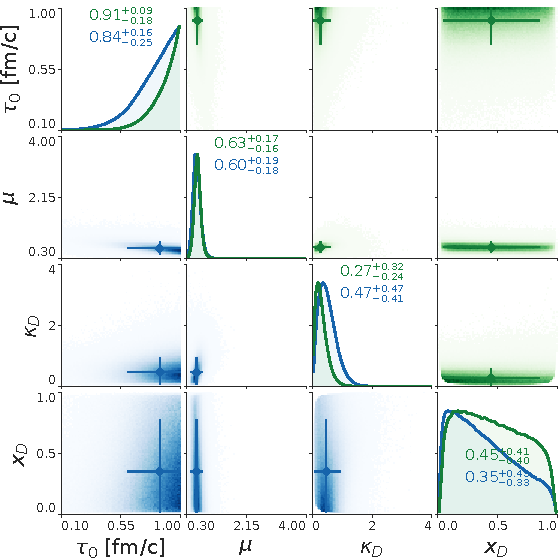
\includegraphics{posterior}
  \caption{Posterior distributions of the model parameters, listed in Table~\ref{tab:parameters}, for the relative-skewness (blue lower diagonal) and absolute-skewness (red upper diagonal) models. The diagonal panels are the marginal likelihood distributions of individual model parameters, while off-diagonal panels are joint distributions for pairs of model parameters.}
  \label{fig:posterior}
\end{figure*}

\subsection{Posterior distribution of model parameters}
Fig.~\ref{fig:posterior} presents the Bayesian posterior probability distributions for the relative- and absolute-skewness models (blue lower- and red upper-triangular matrices respectively).
Diagonal panels show the marginal posterior distribution of individual model parameters (all other parameters integrated out), while off-diagonal panels show the joint distribution for pairs of model parameters, reflecting their correlations.

The posterior distributions contain a wealth of information; here we summarize a few key observations:
\begin{itemize}[itemsep=0pt, leftmargin=2\parindent]
  \item Both models prefer the entropy deposition parameter $p$ close to $0$, consistent within the range of the prior distribution extracted from {Bernhard:2016tnd}.
  \item The p+p multiplicity fluctuation parameter is well constrained and distributed about $k=2.0$ for both models.
    These $k$ values are also consistent with the range of the previous estimates obtained from fits to p+p, p+Pb, and Pb+Pb multiplicity distributions at midrapidity {Moreland:2014oya}.
  \item The relative-skewness model prefers a larger nucleon width than the absolute-skewness model. 
  For future studies, one may also use more granular protons with subnucleonic structure instead of Gaussian protons.
  \item The calibrated relative-skewness model exhibits almost zero shift about the mean and large skewness, while the absolute-skewness model prefers a shift close to the center-of-mass rapidity and a moderate skewness. 
\end{itemize}
Superficially, it appears that the models prefer qualitatively different mechanisms for longitudinal entropy deposition; however, for realistic values of the nuclear thickness function in heavy-ion collisions, the behavior of the two calibrated models is nearly identical, despite the use of two possible skewness parametrizations, as is shown in Fig.~\ref{fig:post_dsdy}.
The lines and bands in Fig.~\ref{fig:post_dsdy} correspond to the mean and $1\sigma$ uncertainty of the calibrated models predictions. 
We vary the nuclear thickness functions $T_A$ and $T_B$ from $0.2~\text{fm}^{-2}$ to $2.6~\text{fm}^{-2}$. The maximum of the nuclear thickness function for a Pb nucleus in an optical Glauber model is about $2.2~\text{fm}^{-2}$. However, the event-by-event $T_A$ and $T_B$ may exceed this value in the presence of nucleonic fluctuations.
The calibrated relative- and absolute-model predictions agree within $1\sigma$ uncertainty band.
This observation has an important implication.
The two models adapt their parameters independently to describe the data and they coincide on one functional form of initial entropy deposition in terms of $T_A$ and $T_B$.
Therefore, with experimental inputs from the charged particle pseudorapidity densities and two-particle pseudorapidity correlations, a systematic model-to-data comparison can extract the form of the three-dimensional initial entropy distribution for relativistic heavy-ion collisions at the LHC.

\begin{figure}
  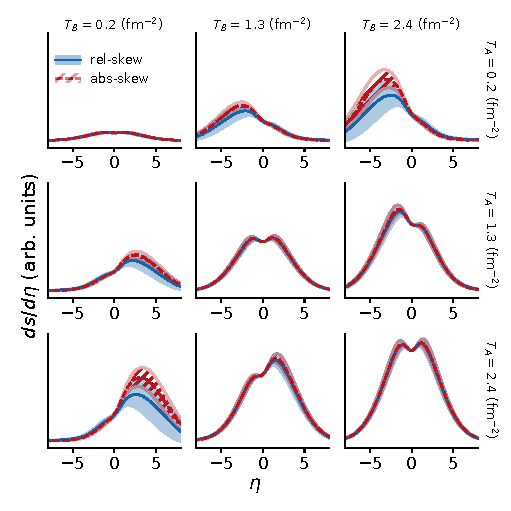
\includegraphics{post_dsdy}
  \caption{Applying parameters sampled from the posterior probability distribution to Eq.~\eqref{cgf} along with Eq.~\eqref{regulateEq}, this plot shows the resulting local entropy profile $ds/d\eta$ varying $T_A$ and $T_B$ from $0.2~\text{fm}^{-2}$ to $2.6~\text{fm}^{-2}$. The lines are the mean predictions and the bands denote $1\sigma$ model uncertainties.
  }
  \label{fig:post_dsdy}
\end{figure}


\subsection{Predictions for novel observables}
Both the relative- and absolute-skewness models provide comparable descriptions of multiplicity observables in p+Pb and Pb+Pb collisions which makes sense given that they predict effectively identical three-dimensional initial entropy profiles when calibrated to fit experimental data.
In this section, we proceed to investigate whether they can describe azimuthally sensitive observables such as flows, event-plane decorrelations and symmetric cumulants, and for completeness, we shall conduct the calculation with both models.
Here we use selected initial condition parameters around the peaks of the posterior distributions for each model (Table \ref{tab:chosen_parameters}) and perform viscous 3+1D hydrodynamic evolution with UrQMD as an afterburner.
These observables are a nontrivial test of the proposed model as they resolve azimuthal correlations which have not been included in the calibration process.

\begin{table}[t]
  \caption{Selected high-probability parameter sets}
    \begin{tabular}{lll}
      Parameter & rel-skew	& abs-skew \\
      \paddedhline
      $N_{\textrm{Pb+Pb}}^\dagger$   & 150.0     & 154.0  \\
      $p$	    & 0.0      & 0.0  \\
      $k$	    & 2.0     & 2.0  \\
      $w$	    & 0.59     & 0.42  \\
      $\mu_0$   & 0.0     & 0.75  \\
      $\sigma_0$ & 2.9    & 2.9  \\
   	  $\gamma_0$ & 7.3		& 1.0	\\
      $J$	     & 0.75 & 0.75	\\
    \end{tabular}
  \raggedright{$\dagger$ Normalization tuned with ideal hydro is reduced when using viscous hydro.}
  \label{tab:chosen_parameters}
\end{table}

\subsection{Anisotropic flows} 
As a preliminary check, we first verify that previous results for the elliptic and triangular flow harmonics $v_2\{2\}$ and $v_3\{2\}$ obtained using \trento\ initial conditions at midrapidity {Bernhard:2016tnd} are indeed recovered by the rapidity-dependent model extension.
Fig.~\ref{fig:vn_cen} shows the centrality dependence of $p_T$-integrated flow for ${0.2  < p_T < 5.0}$~GeV and $|\eta| < 0.8$ calculated from the \emph{three-dimensional} hybrid model compared to \mbox{ALICE} measurements {Adam:2016izf} using the  $Q$-cumulant method {Bilandzic:2010jr}.
The 3+1D hydrodynamics code used in this study only partially implements bulk viscous corrections and thus is not yet suitable for quantitative calculations involving finite bulk viscosity.
We therefore assert a QGP specific bulk viscosity $\zeta/s = 0$ which precludes direct comparison with the boost-invariant VISH2+1 hydrodynamics code {Song:2007ux, Shen:2014vra, Bernhard:2016tnd} and the corresponding shear and bulk viscosities determined by the previous Bayesian analysis {Bernhard:2016tnd}.
For the QGP specific shear viscosity, we choose constant QGP $\eta/s = 0.17$ and $0.19$ for relative- and absolute-skewness models respectively, which provide good descriptions of the data {Gale:2012rq, Niemi:2015qia}, although it is not a systematic best fit.
The resulting $v_2\{2\}$ and $v_3\{2\}$ agree with experimental data within $10\%$ and verify that the generating function rapidity extension recovers previous \trento\ initial condition results at midrapidity.

\begin{figure}
  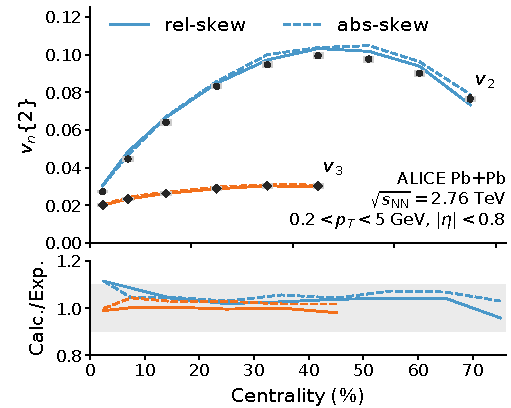
\includegraphics{vn_cen}
  \caption{Elliptic and triangular flow cumulants $v_2\{2\}$ and $v_3\{2\}$ as a function of centrality calculated from 3+1D hybrid model simulations using constant specific shear viscosity $\eta/s=0.17$ and $0.19$ for relative- and absolute-skewness models respectively, zero bulk viscosity $\zeta/s=0$ and hydro-to-micro switching temperature $T_\text{sw}=154$~MeV.
  The initial condition parameters are selected from the Bayesian posterior.}
  \label{fig:vn_cen}
\end{figure}

We now proceed to calculate the pseudorapidity-dependent flows which provide a sensitive handle on the QGP transverse structure at different rapidity values.
The ALICE collaboration has measured $v_n\{2\}(\eta)$ and $v_2\{4\}(\eta)$ within the wide pseudorapidity interval $-3.5 < \eta < 5.0$ and extrapolated to zero $p_T$ {Adam:2016ows}. 
This extrapolation reduces integrated flow relative to measurements with a nonzero $p_T$ cut because it averages over low-$p_T$ particles which generally have less flow.
The same behavior occurs in hydrodynamic models, although models which mispredict mean $p_T$ also mispredict the corresponding change in flow produced by introducing a $p_T$ cut.
The hybrid model used in this study omits bulk viscous corrections and thus overpredicts mean $p_T$.
This means it cannot describe hydrodynamic flow measurements with different $p_T$ cuts using a single value of $\eta/s$.
To circumvent this issue, we use $\eta/s=0.25$--$0.28$ when comparing to ALICE measurements that are extrapolated to zero $p_T$. 
Future implementation of realistic bulk viscous corrections would eliminate such fine tuning.

The pseudorapidity-dependent flows are estimated using the cumulant approach {Bilandzic:2010jr}, where particles of interests (POI) are correlated with reference particles.
The differential flow is then calculated via,
\begin{eqnarray}
v_n^\prime\{2\} = \frac{d_n\{2\}}{\sqrt{c_n\{2\}}},\\
v_n^\prime\{4\} = \frac{-d_n\{4\}}{\left(-c_n\{4\}\right)^{3/4}},
\end{eqnarray}
where $d_n\{2\}$, $d_n\{4\}$ is the two- and four-particle cumulants between the POI and reference particles and $c_n\{2\}$ and $c_2\{4\}$ are the cumulants among reference particles.
For POI with $\eta > 0$ ($\eta < 0$), the reference particles are restricted to $-0.8 <\eta < 0$ ($0 <\eta < 0.8$) to avoid autocorrelations.
The results are shown in the left panel of Fig.~\ref{fig:vn_eta} for nine centrality classes.
The correlation functions $d_n(\eta)$ and $c_n(\eta)$ are symmetrized since the event-averaged pseudorapidity-differential flow for the Pb+Pb system should be invariant with respect to the substitution $\eta \rightarrow -\eta$.

Both models predict $v_2\{2\}$, $v_2\{4\}$ and $v_3\{2\}$ that decrease from mid to forward/backward rapidity and produce a triangle shaped structure as measured by ALICE.
Incidentally, the absolute-skewness model agrees with experiment slightly better at large pseudorapidity.
It has been realized that the slope of $v_n(\eta)$ which produces this triangular shape is highly sensitive to the hadronic shear viscosity {Denicol:2015bnf}, and thus Fig.~\ref{fig:vn_eta} corroborates that UrQMD provides a semi-quantitative description of hadronic viscosity below the QGP transition temperature.
However, for central to mid-central collisions, the slope of the decreasing $v_2$ as a function of pseudorapidity is underpredicted, resulting in a flatter $v_n(\eta)$ than the experiments.
The reason for this discrepancy may be complicated.
Apart from improving initial conditions, a realistic bulk viscosity and a temperature dependent specific shear viscosity should definitely affect the results.
Another reason could be the use of the QCD EoS and QGP transport coefficient $\eta/s$ in the limit of vanishing baryon chemical potential, which may not be a good approximation at large pseudorapidity even at LHC energies.

\begin{figure*}
  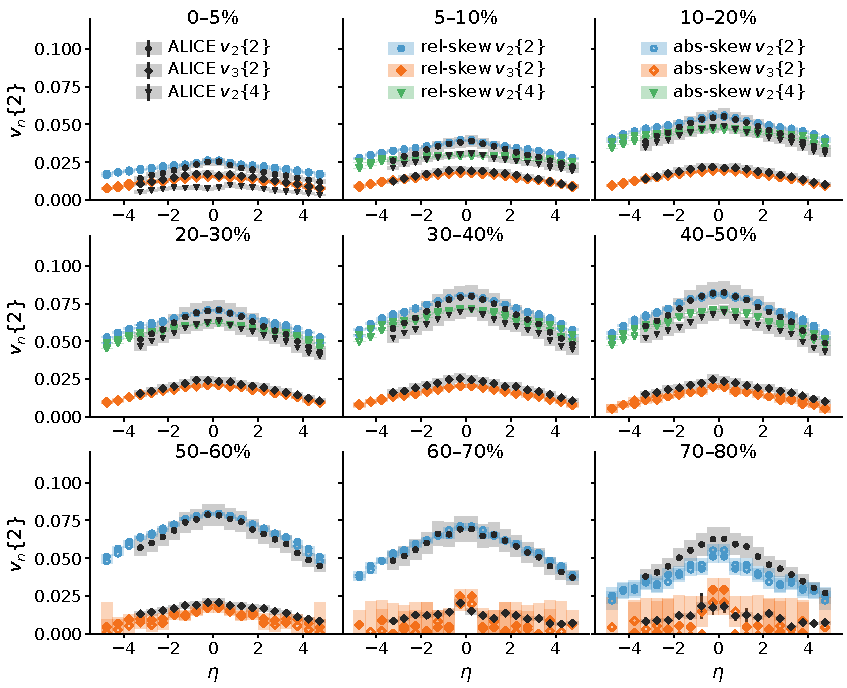
\includegraphics{vn_eta}
  \caption{Pseudorapidity dependence of anisotropic flow coefficients $v_2\{2\}$, $v_3\{2\}$ and $v_2\{4\}$ (blue circle, green triangle and orange diamond shaped symbols) calculated from the hybrid model with constant specific shear viscosity $\eta/s=0.25$ and $0.28$ for relative- and absolute-skewness models respectively (solid and open symbols), compared to data from ALICE (smaller black symbols) with $p_T > 0$~GeV (extrapolated) in different centrality bins. 
  The bands for each theory calculation point indicate $1\sigma$ statistical error, while experimental bands/bars denote $1\sigma$ systematic and statistical errors respectively.}
  \label{fig:vn_eta}
\end{figure*}



\begin{figure*}
  \begin{center}
  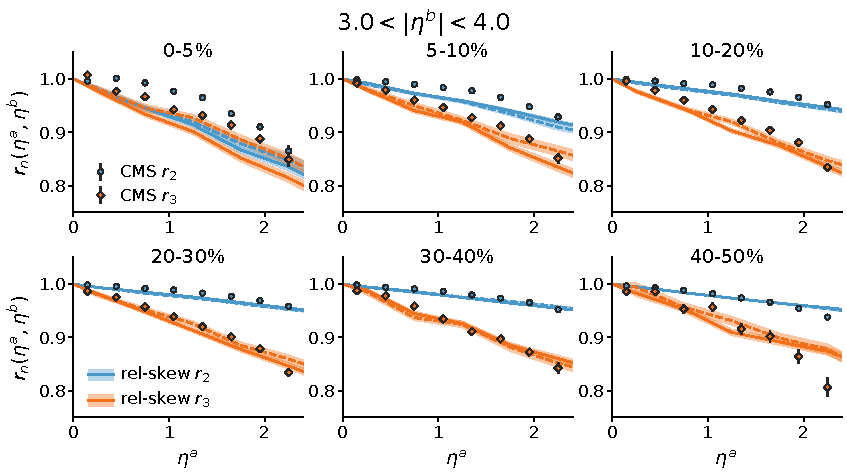
\includegraphics{evt_pln_decorr_near}
  \quad\quad\quad
  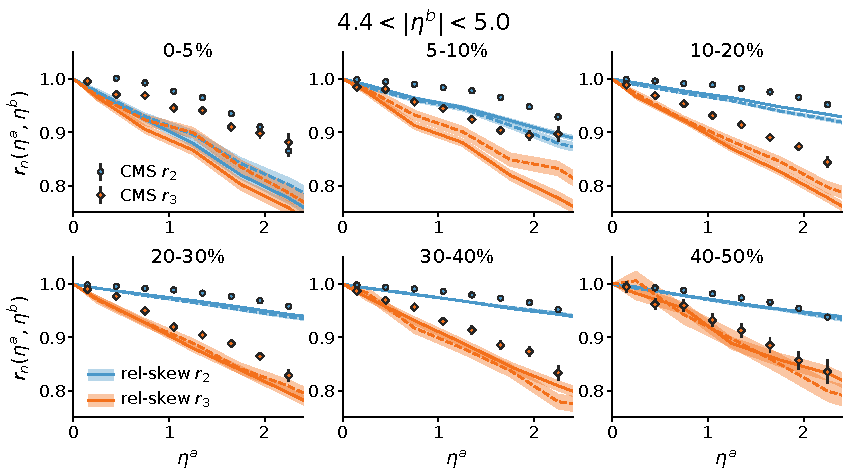
\includegraphics{evt_pln_decorr_far}
  \end{center}
  \caption{Left: The event-plane decorrelation for $n=2,3$ in different centrality bins with the reference particles from $3.0<|\eta^b|<4.0$.
  Right: The same quantities as the left panel but with the reference particles from $4.4<|\eta^b|<5.0$. 
  Theory bands indicate $1\sigma$ statistical error, while experimental bands/bars denote $1\sigma$ systematic and statistical errors respectively.}
  \label{fig:epd}
\end{figure*}


\subsection{Event-plane decorrelation}

Next, we study the event-plane decorrelation as a function of pseudorapidity using the calibrated relative-skewness model. 
The event planes are defined by the angles
\begin{equation}
  \Psi_n^\text{EP} = \frac{\text{atan2}(\langle \sin n \phi \rangle, \langle\cos n \phi \rangle)}{n},
\end{equation}
where the average is performed over particles of interest.
In general, the angles $\Psi_n^\text{EP}$ may change as a function of pseudorapidity due to longitudinal initial state fluctuations and finite particle effects.
As a consequence, two event-plane angles constructed from sets of particles separated by a finite rapidity gap will decorrelate as the rapidity gap increases.
This effect is important as it affects not only the calculation of soft observables involving a finite pseudorapidity gap or a large pseudorapidity interval, but also the interpretation of hard probe observables where particles from a rare hard process are often correlated with reference particles from different pseudorapidity bins.
It has been studied in a number of previous works including a longitudinally torqued fireball model with fluctuating sources {Bozek:2015bna}, AMPT calculations which studied its influence on flow observables {Jia:2014ysa, Xiao:2012uw}, as well as coarse-grained AMPT initial conditions that were embedded in 3+1D ideal hydrodynamic simulations {Pang:2015zrq}.

The decorrelations receive contributions from both random fluctuations during the evolution process and the systemic twist of the participant plane arising from initial longitudinal fluctuations {Bozek:2015bna}.
In the present parametric initial condition model, the participant plane twist arises naturally from local longitudinal fluctuations.
The transverse geometry at forward (backward) space-time rapidity is dominated by the projectile (target) participant density.
As a result, the participant plane gradually interpolates between the projectile and target densities, leading to a systemic twist in the beam direction.
The time evolution also contributes to decorrelation among the event-planes.
For example, early- and late-stage dynamics introduce additional fluctuations that partially randomize event-plane orientations.
Stochastic contributions from pre-equilibrium dynamics are neglected in the present study, but fluctuations in the hadronic phase are naturally accounted for by the UrQMD transport model.

The CMS collaboration has measured the event-plane decorrelations in Pb+Pb collisions using the $\eta$-dependent factorization ratio $r_n(\eta^a, \eta^b)$ {Khachatryan:2015oea}, defined as
\begin{align}
  r_n(\eta^a, \eta^b) &= \frac{V_{n\Delta}(-\eta^a, \eta^b)}{V_{n\Delta}(\eta^a, \eta^b)}, \\
  V_{n\Delta}(\eta^a, \eta^b) &= \langle\langle \cos(n\Delta\phi) \rangle\rangle,
\end{align}
where the double average means averaging over particles in each event and then averaging over all events in a given centrality class. 
The use of three $\eta$-bins ($\pm \eta^a$ and $\eta^b$) reduces short range correlations.
The ratio $r_n(\eta^a, \eta^b)$ reflects the fluctuation of event-plane angles separated by $\eta^a+\eta^b$ relative to the fluctuation of angles separated by  $|\eta^a-\eta^b|$ {Khachatryan:2015oea}.

We compare our calculation to the CMS measurements with both $3.0 < \eta^b < 4.0$ and $4.4 < \eta^b < 5.0$ and momentum cuts $p_T^b > 0$~GeV and ${0.3 < p_T^a < 3.0}$~GeV.
The $\eta$-dependent factorization ratios $r_2$ and $r_3$ for six centrality classes and different $\eta^b$ cuts are shown in Fig.~\ref{fig:epd}.
Both models predict a prominent $n=2, 3$ event-plane decorrelation in central collisions which decreases with increasing centrality.
For midcentral collisions, the nuclear geometry largely defines the $n=2$ participant plane---fluctuations and twisting are perturbations around this predominant direction---and hence $r=2$ decorrelation is reduced.
On the other hand, the $n=3$ event-plane receives little contribution from the nuclear geometry but is dominated mostly by fluctuations; it therefore has a similar slope over all six centralities.
In central collisions, the contribution from nuclear geometry is overwhelmed by fluctuations leading to similar $n=2$ and $n=3$ decorrelations.
The calculations describe the observed $n=2,3$ event-plane decorrelations with $3.0 < \eta^b < 4.0$ very well except the most central $0$--$5\%$ centrality, but systematically overpredict the magnitude of the decorrelations with $4.4 < \eta^b < 5.0$, especially for $0$--$10\%$ central collisions.
The reason is that the model, by construction, extends well-developed mid-rapidity initial conditions to finite pseudorapidity. 
Even though it is calibrated to multiplicity observables, it gradually loses its predictive power for fine-structure flow observables when moving far away from mid-rapidity.
Specifically, the model predicts decorrelations between the event-planes that are stronger for larger $\eta^b$ bins, while the experiment sees that the magnitude of decorrelation saturates when moving from $3.0<\eta^b<4.0$ to $4.4<\eta^b<5.0$.
Future improvements to the model at large pseudorapidity are clearly needed.
Nevertheless, the model's explanation of the event-plane decorrelations for $3.0 < \eta^b < 4.0$ remains nontrivial.
Both models were both calibrated with $\dnchdy$ and rms $a_1$ data.
These multiplicity observables do not constrain the transverse structure of the event at different pseudorapidities, and hence reproducing $r_2$ and $r_3$ means the calibrated initial condition models not only reproduce global longitudinal entropy deposition and fluctuations, but also capture features of the longitudinal dependence of transverse geometry within $|\eta| \lesssim 4$.


\begin{figure*}
  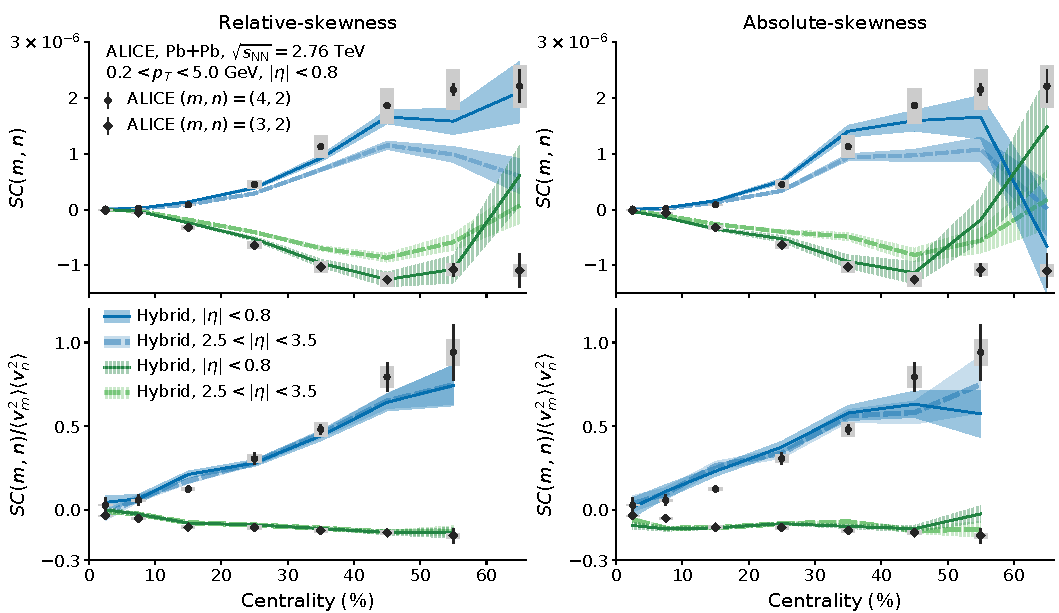
\includegraphics{smn}
  \caption{Top row: calculated $SC(4,2)$ and $SC(3,2)$ as functions of centrality compared to ALICE measurements, with the same 3D hybrid model set-up as used for Fig. \ref{fig:vn_cen}.
  We conduct calculations in two kinematic ranges: $|\eta|<0.8$ is the pseudorapidity cut used by current the ALICE measurement and $2.5<|\eta|<3.5$ is our prediction for the symmetric cumulants away from mid-rapidity in the Pb+Pb system.
  Bottom row: $SC(m,n)$ normalized by $\langle v_m^2\rangle\langle v_n^2\rangle$ for two two kinematic ranges.
  The left column and right column show results using relative- and absolute-skewness respectively.
   }
  \label{fig:smn} 
\end{figure*}


\subsection{Flow correlations}

Correlations between different anisotropic flow harmonics can be used to further constrain the initial state geometry {Niemi:2012aj}.
Experimentally, these correlations can be quantified using either event shape engineering {Schukraft:2012ah, Aad:2015lwa} or the symmetric cumulants $SC(m,n)$ {Bilandzic:2013kga}. 
Here we focus on the symmetric cumulants which are defined as,
\begin{align}
SC(m, n) &= \langle\langle \cos(m\phi_1+n\phi_2-m\phi_3-n\phi_4)\rangle\rangle \nonumber \\
\nonumber &- \langle\langle\cos[m(\phi_1-\phi_2)]\rangle\rangle\langle\langle\cos[n(\phi_1-\phi_2)]\rangle\rangle \label{eq:scmn}\\
&= \langle v_m^2 v_n^2 \rangle - \langle v_m^2\rangle\langle v_n^2\rangle.
\end{align}
The centrality dependences of $SC(4,2)$ and $ SC(3,2)$ at midrapidity have recently been measured by ALICE {ALICE:2016kpq}. 
A positive value of $SC(m,n)$ means that a large $v_m$ is more likely to be observed with a large $v_n$, while for negative values of $SC(m,n)$, a large $v_m$ favors small $v_n$.
The symmetric cumulants $SC(m,n)$ are nearly insensitive to nonflow effects while remaining sensitive to collective effects, initial geometry fluctuations $\langle \varepsilon_m^2 \varepsilon_n^2 \rangle - \langle \varepsilon_m^2 \rangle \langle \varepsilon_n^2 \rangle$ and the QGP specific shear viscosity {ALICE:2016kpq, Zhu:2016puf}.
To remove its dependence on the magnitudes of $\langle v_m^2\rangle$ and $\langle v_n^2\rangle$, we also calculate the normalized symmetric cumulants
\begin{equation}
  NSC(m,n) = SC(m,n)/\langle v_m^2\rangle\langle v_n^2\rangle.
\end{equation}
Here we use this tool to not only study the flow correlations at midrapidity, but also reveal its pseudorapidity dependence.

Fig.~\ref{fig:smn} shows the calculated symmetric cumulants compared to ALICE measurements using the relative- and absolute-skewness models with the same transport coefficients as in Fig.~\ref{fig:vn_cen}. 
We use the same centrality bins as ALICE experiments and the centrality averaged symmetric cumulants are performed with a multiplicity weight as discussed in {Gardim:2016nrr}.
We first calculate $SC(4,2)$ and $SC(3,2)$ at midrapidity $|\eta|<0.8$ (solid lines) to match the rapidity cuts of the ALICE measurement.
The negative $SC(3,2)$ is a result of initial eccentricity correlations, while the large positive $SC(4,2)$ is produced by nonlinear correlations between $v_2$ and $v_4$ during the medium evolution {Giacalone:2016afq, Qian:2016fpi, Bhalerao:2014xra, Zhou:2015eya}.
The resulting symmetric and normalized symmetric cumulants agree with the data quite well and support previous constraints on the QGP initial conditions at midrapidity {Bernhard:2016tnd}. 

Next, we shift our attention away from midrapidity and predict the symmetric (normalized symmetric) cumulants in the rapidity interval $2.5 < |\eta| < 3.5$ (dashed lines) which has not been measured.
In this calculation, we take two reference particles from $|\eta| < 0.8$ and two POI from $2.5 < |\eta| < 3.5$ and calculate
\begin{align}
SC^\prime(m, n) &= \langle\langle \cos(m\phi_1+n\phi_2-m\phi_3^\prime-n\phi_4^\prime)\rangle\rangle \\
\nonumber &- \langle\langle\cos[m(\phi_1-\phi_2^\prime)]\rangle\rangle\langle\langle\cos[n(\phi_1-\phi_2^\prime)]\rangle\rangle, \label{eq:scmn}
\end{align}
where the primed symbols represents the azimuthal angle of POI.
Magnitudes of both $SC^\prime(4, 2)$ and $SC^\prime(3, 2)$ are significantly suppressed at forward/backward rapidities, in accordance with the behavior of $v_2\{2\}(\eta)$ and $v_3\{2\}(\eta)$ as presented in the text in Fig.~\ref{fig:vn_eta}.
However the normalized symmetric cumulants $NSC^\prime(4,2)$ and $NSC^\prime(3,2)$ are consistent within uncertainty bands for different pseudorapidity cuts.
We observe that the normalized symmetric cumulant does not change as a function of psuedorapidity for either the relative- or absolute-skewness model and hence expect it to remain constant in nature as well.
Future comparison with available data should correspondingly impose strong constraints on our approach for modeling the three-dimensional initial conditions.


In summary, we have proposed a new method to extend arbitrary initial condition models defined at midrapidity to forward and backward pseudorapidity.
The method describes initial entropy deposition as a purely local function of nuclear participant densities, with the longitudinal profile reconstructed from generating-function cumulants.
The first three cumulants of the distribution (mean, standard deviation, and skewness) are included.
We set the mean proportional to the center-of-mass rapidity of local nuclear participant densities, and parametrize the standard deviation using a constant rapidity width.
Two models for the distribution's skewness are investigated: one where the skewness is proportional to the relative nuclear thickness difference, and one where it is proportional to the absolute difference.

We apply the method to extend the parametric \trento\ initial condition model which has been previously used to constrain QGP initial conditions and medium properties at midrapidity. 
The resulting three-dimensional models are then calibrated using Bayesian parameter estimation to fit p+Pb and Pb+Pb charged particle pseudorapidity densities $\dnchdy$ and the root-mean-square of the two particle pseudo-rapidity correlation's Legendre decomposition coefficient $a_1$ at the LHC.
After the calibration, both models provide comparable descriptions of experimental $\dnchdy$ and rms $a_1$ data.
Despite the apparent difference in the skewness ansatz, the calibrated models predict effectively the same behavior for local longitudinal entropy deposition as function of nuclear thickness in heavy-ion collisions.

Using the calibrated relative- and absolute-skewness initial condition models, we study pseudorapidity-dependent anisotropic flows, event-plane decorrelations and flow correlations in Pb+Pb collisions.
The model nicely describes integrated flows $v_2$ and $v_3$ at midrapidity as well as the pseudorapidity dependence of differential flow for different centrality classes.
The elliptic and triangular event-plane decorrelations with $3.0 < |\eta^b| < 4.0$ are well explained except for the most central collisions, but both models overpredict the decorrelations with the reference particles $4.4 < |\eta^b| < 5.0$.
This is because the model is an extension from mid-rapidity calculation and it gradually loses its accuracy at large forward/backward rapidity.
Both models give a satisfactory description of flow correlation $SC(3,2)$ and $SC(4,2)$ at midrapidity, which can be used to predict their values at forward/backward pseudorapidity where their values have not yet been measured.

The present work expands upon previous efforts to parametrize and constrain local initial condition properties using global final-state observables.
We show that these local properties are overconstrained by multiplicity observables alone and can be reverse engineered using systematic model-to-data comparison with quantitative uncertainty.
Specifically, it is a first attempt to use data-driven methods to infer what the entropy density distribution looks like at the hydrodynamic starting time in all three spatial dimensions.

It is clear that local forward/backward fluctuations are responsible for a variety of longitudinally sensitive phenomena beyond mere multiplicity fluctuations.
The general agreement of the present framework with pseudorapidity dependent flows and event-plane decorrelations corroborates the use of relativistic viscous hydrodynamics in describing the QGP dynamics away from midrapidity region.
The resulting knowledge can then be used to provide direct feedback for first-principle calculations of the QGP initial conditions, and can also be applied to studies where the QGP initial conditions act as a nuissance parameter, e.g.\ when modeling the propagation of hard probes through the medium in order to measure their response.

The present analysis would benefit from a number of future improvements.
For example, it would be interesting to add subnucleonic structure to the nuclear thickness functions in order to examine its effect on longitudinal rapidity fluctuations.
Also, in this work we assume that the multiplicity observables are insensitive to viscous effects and use ideal hydrodynamics in the model-to-data comparison process.
In the calculation of flow observables, we use an over-simplified constant specific shear viscosity and zero bulk viscosity, although there have been many works suggesting preference for a temperature dependent shear viscosity and finite bulk viscosity {Bernhard:2016tnd,Niemi:2015qia, Ryu:2015vwa}.
We leave these refinements to future work and hope the calibrated initial conditions presented in this study provide a more realistic description of the three-dimensional structure of relativistic heavy-ion collisions which will prove useful in constraining the properties of hot and dense QCD matter.